\subsection{Universal adversarial training}

\setlength\parindent{0pt}

In this section we test the performance of the same network, trained using three different methods, against perturbation based attacks. This is in the hope of validating the results of Shafahi et al \cite{shafahi_universal_2018}, as well as generating new ideas of how to come up with defences.

\subsubsection{Layout}

We have decided to run our simulations in python using the PyTorch package. We run tests on the MNIST data set of hand written digits \cite{lecun2010mnist}. These are gray-scale $28 \times 28$ images depicting the digits 0-9. The training set contains 60000 of those images, while the test set contains 10000 images. We use three different training methods:

\begin{itemize}
	\item vanilla training (with no defence against perturbation),
	\item universal adversarial training (as set out in \cite{shafahi_universal_2018}) and Algorithm \ref{Alg_3}, and
	\item trained as described in Algorithm \ref{Alg_4}.
\end{itemize}

We will test the trained networks against two types of attacks: FGSM and a universal adversarial attack.

\subsection{Code description}

All the code for this project can be found with the report, along with the trained models we used to generate the results within this report.\\ 

% There will be two network architectures used in this project, one for the image classifiers and one to generate perturbations for the sake of attacking. The image classifier has the following layers

% \begin{enumerate}
% 	\item 1st convolution layer, with kernel size 5 and extracting 10 features,
% 	\item 2nd convolution layer, with kernel size 5 and extracting 20 features,
% 	\item one layer of 50 nodes applying a ReLU, and
% 	\item an application of softmax to give a single classification output.
% \end{enumerate}

% For the perturbation generator we simply have the following architecture

% \begin{enumerate}
% 	\item it has two layers of $28 \times 28 = 784$ nodes each applying ReLU, and
% 	\item clamping the values between 0 and $\epsilon$ (the max perturbation size set by the user) to provide an output image of $28 \times 28$.
% \end{enumerate}

Throughout this section we focus on using the LeNet-5 architecture \cite{lecun1998gradient}, but we encourage the reader to experiment with different architectures. The models are updated as described in Section \ref{sec:uniadvtrain}, using inbuilt PyTorch functions.\\

Within the training a number of variables are chosen

\begin{enumerate}
	\item The learning rate $\tau$, how far in the direction of the steepest decent we move.
	\item How much the attackers are allowed to perturb the image (in form of the norm bound $\varepsilon$).
	\item The cap for the loss function, see \cite{shafahi_universal_2018} for further details.
	\item The momentum within the learning, how much it gets effected by the new change in direction.
	\item The number of times one runs through the entire training data.
\end{enumerate}

These values are fixed for the results, please see the code for details. These values are chosen using trial and error in hopes to get the most meaningful output. We encourage the reader to further experiment and follow best practices to avoid over fitting.

\subsubsection{Results of model}
In Figure \ref{fig:sample_pertubations} we visualise sample images of the MNIST dataset together with trained universal perturbations based on Algorithm \ref{Alg_3} and Algorithm \ref{Alg_4}. Note that for consistency we use - instead of the FGSM-inspired update rule - the same update rule for the perturbation in Algorithm \ref{Alg_3} that we use in Algorithm \ref{Alg_4}.
\begin{figure}[!h]
    \centering
    \begin{subfigure}[c]{0.3\textwidth}
    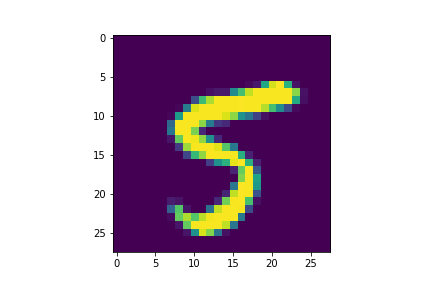
\includegraphics[width=\textwidth]{attack_image.png}
    \caption{Sample image}
    \label{subfig:my_label1}
    \end{subfigure}
    \begin{subfigure}[c]{0.3\textwidth}
    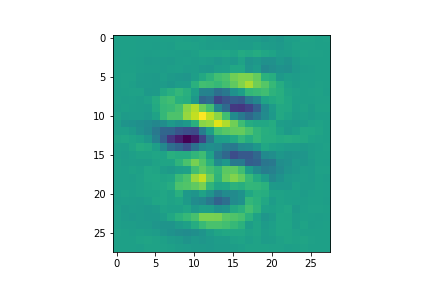
\includegraphics[width=\textwidth]{attack_perturbation.png}
    \caption{Universal perturbation}
    \label{subfig:my_label2}
    \end{subfigure}
    \begin{subfigure}[c]{0.3\textwidth}
    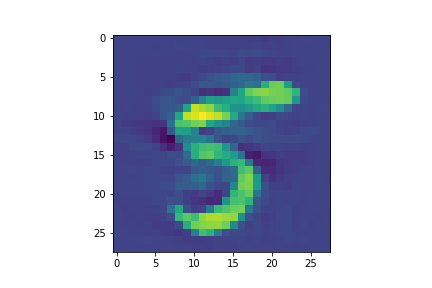
\includegraphics[width=\textwidth]{attack_perturbed_image.png}
    \caption{Perturbed sample image}
    \label{subfig:my_label3}
    \end{subfigure}\\
    \begin{subfigure}[c]{0.3\textwidth}
    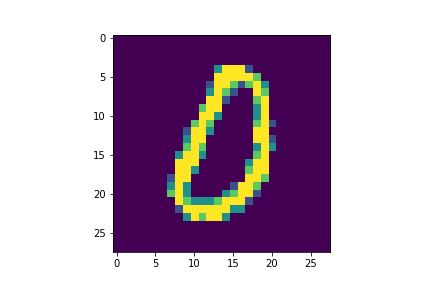
\includegraphics[width=\textwidth]{attack_defence_image.png}
    \caption{Sample image}
    \label{subfig:my_label4}
    \end{subfigure}
    \begin{subfigure}[c]{0.3\textwidth}
    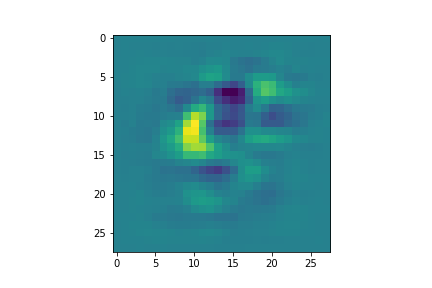
\includegraphics[width=\textwidth]{attack_defence_perturbation.png}
    \caption{Universal perturbation}
    \label{subfig:my_label5}
    \end{subfigure}
    \begin{subfigure}[c]{0.3\textwidth}
    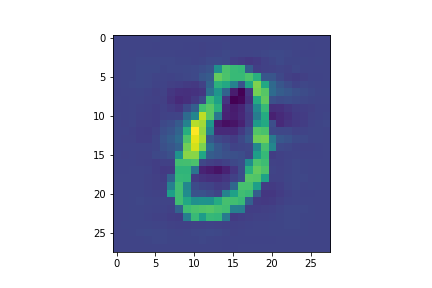
\includegraphics[width=\textwidth]{attack_defence_perturbed_image.png}
    \caption{Perturbed sample image}
    \label{subfig:my_label6}
    \end{subfigure}
    \caption{This figure shows a generic input from the MNIST training dataset (Figure \ref{subfig:my_label1}), a universal perturbation computed with Algorithm \ref{Alg_3} and a modified update rule for the perturbation (Figure \ref{subfig:my_label2}) as well as the perturbation added to the input \ref{subfig:my_label3}. Figure \ref{subfig:my_label4}-\ref{subfig:my_label6} show the same quantities for Algorithm \ref{Alg_4}.}
    \label{fig:sample_pertubations}
\end{figure}

In general, our experiments showed that the vanilla model performed best on the training data (95\% accuracy), with the universal adversarial trained model (87\% accuracy) and the AI trained model (81\% accuracy) performing worse. The results of the FGSM attack are noted below. Epsilon is the size of the perturbation.

\begin{figure}[!ht]
\centering
	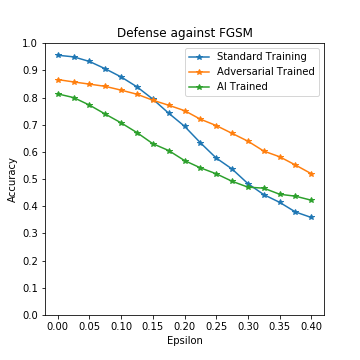
\includegraphics[scale=0.5]{Advsarial_code/figures/doc_defense_against_FGSM.png}
	\caption{FGSM attack - Size of perturbation against accuracy of models.}
\end{figure}

Although initially the Vanilla model outperforms the other two models, given large enough perturbation the other models are more stable against FGSM attack.\\ 

When being perturbed by a universal adversarial attack the vanilla model always out preformed the models trained with defences against this exact attack. 

\begin{figure}[!ht]
\centering
	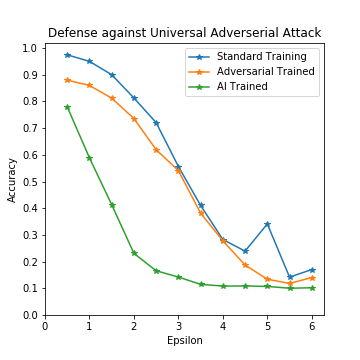
\includegraphics[scale=0.5]{Advsarial_code/figures/doc_defense_against_UAA.png}
	\caption{Universal adversarial attack - Size of perturbation against accuracy of models.}
\end{figure}

However, this could easily be caused by the wrong choice of variables, architecture, or that the models without defence converges quicker than those with defences.

%\subsubsection{Further Ideas}

%An idea we did not have time to implement was to use genetic algorithms to test different defence an attacking algorithms. The idea would be to pair image classifiers with a perturbation generators and then see how the pairs fair against one another, equip a score then breed these alogorithms. 
